\documentclass[../../main]{subfiles}
\graphicspath{{\subfix{../../Images/}}}

\begin{document}

% TODO: Przed napisaniem tej części zastanawiałem się, jak podzielić miedzy sobą pojęcia
%architektury, struktury i pojęcia z języka angielskiego - desing. Dlaczego? No bo conajmniej pierwsze
%dwa pojęcia będą często używane w tej prace, i ja się obawiałem, że będę wykorzystywał je w własny,
%niezdefiniowany sposób (bo nie znalazłem tak naprawdę dokładnej definicji, są tylko dyfinicje dla
%poszczególnych branży, w których te pojęcia są używane).
%Po przemyśleniu zdefiniowałem ję w następujący sposób:
%Struktura - łączenie czegokolwiek posiadającego własciwości lub funkcjanolności jednego typu z
%czymkolwiek posiadającym właściwości lub funkcjanolności takiego samego typu w określony
%sposób dla stworzenia czegokolwiek z innymi właściwościami lub funkcjanolnościami.
%Architektura - łączenie czegokolwiek posiadającego własciwości lub funkcjanolności jednego typu
%z czymkolwiek posiadającym właściwości lub funkcjanolnościinnego typu w określony sposób dla
%stworzenia czegokolwiek z innymi właściwościami lub funkcjanolnościami.
%Design - struktura lub architektura stowrzona dla osiągniecia pewnego celu (IMHO najbliższe %tłumaczenie na język Polski - projekt, chociaż w języku angielskim project =/= design).
%Zostawiam to tu, aby nie zgubić. W pracę będę korzystał z tych pojęć zgodnie z tymi definicjami.}

Ten rozdział przedstawia i opisuje architektury oprogramowania w systemach wbudowanych (używana podczas
napisania tej pracy definicja pojęcia "system wbudowany" jest zamieszczona w
\hyperref[sec:zalacznik-1]{załączniku nr 1}) bazujących się na jednostkach obliczeniowych
skonstruowanych na podstawie architektury \acrshort{arm}'owej. Będą też omówione cechy
przedstawionych architektur oraz właściwości je powodujące. Następnie są przedstawione przykładowe
realizacje tych architektur.

Należy też wspomnieć, że \acrshort{arm} przedstawia też technologię TrustZone, która dodaje kilka
możliwych architektur. Skoro celem tej technologii jest bezpieczeństwo — architektury, które ona
wprowadza, nie zostaną tu omówione, są one jednak wkrótce opisane w \hyperref[sec:zalacznik-2]
{załączniku nr 2}.

W dalszej części pracy wspominany będzie termin "wirtualizacja" i terminy pochodne (parawirtualizacja,
wirtualizacja natywna), których wytłumaczenie można znaleźć w \hyperref[sec:zalacznik-3]{załączniku
nr 3}, są w nim także omówione pojęcia separacji, translacji pamięci i przekierowywania przerwań.

Pojęcia przełączenia stanów i przełączenia kontekstu są wyjaśnione w
\hyperref[sec:zalacznik-4]{załączniku nr 4}.

\subsection{Architektura "nagi metal"}
\begin{figure}[h]
    \centering
    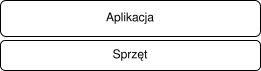
\includegraphics[width=0.55\textwidth]{Images/bare-metal.png}
    \caption{Architektura "nagi metal"}
    \label{fig:bare-metal}
\end{figure}

Najprostsza ze względu na ilość poziomów abstrakcji architektura, składająca się ze sprzętu i aplikacji
wykorzystującej ten sprzęt (\cref{fig:bare-metal}). Dla funkcjonowania (jako system wbudowany) jest
potrzebna jednostka obliczeniowa dla wykonywania poleceń, pamięć dla przechowywania poleceń, moduły
wejścia/wyjścia dla kontaktu ze środowiskiem zewnętrznym i kontroler przerwań dla poinformowania
aplikacji o zdarzeniach z zewnątrz. Zasoby sprzętowe są przydzielane statycznie podczas kompilacji,
nie ma separacji środowisk lub uprzelewanego dostępu. % TODO: uprzelewanego?

Cechy:
\begin{itemize}
    \item Prostota: architektura nie posiada poziomów abstrakcji, aplikacja kontaktuje wprost ze
    sprzętem, nie ma skomplikowanych modułów do zarządzania bezpieczeństwem (np. \acrshort{mmu} lub
    \acrshort{gic});
    \item Wydajność: architektura nie posiada rozbudowanego kodu systemu operacyjnego lub
    hiperwizora, nie ma translacji pamięci i przekierowania przerwań, nie ma przełączania kontekstu;
    \item Determinizm: nie ma konkurencji za zasoby jednostki obliczeniowej przez aplikacje, z powodu
    możliwej obecności tylko jednej aplikacji, pełna gwarancja reakcji na zdarzenie;
\end{itemize}

Uwzględniając powyższe cechy i właściwości, można zrobić wniosek, że taka architektura jest
przeznaczona dla małych jednostek w systemie, np. czujniki, każda z których ma zdefiniowaną jedną cel.
Przykładem realizacji danej architektury może być dowolna aplikacja niewykorzystująca systemu
operacyjnego lub hiperwizora na dowolnej architekturze \acrshort{arm}'owej. Chociaż najczęściej będzie
wybierana jedna z \acrshort{m} architektur, ponieważ są one dla tego najlepiej przeznaczone.

Dana architektura nie stanowi zainteresowania w ramach tej pracy, skoro nie posiada oprogramowania
zarządzającego dostępem do zasobów jednostki obliczeniowej.

\subsection{Architektura z systemem operacyjnym}
\begin{figure}[h]
    \centering
    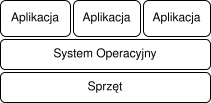
\includegraphics[width=0.55\textwidth]{Images/no-virt.png}
    \caption{Architektura z systemem operacyjnym}
    \label{fig:no-virt}
\end{figure}

Architektura posiadająca jedną warstwę abstrakcji — system operacyjny (\cref{fig:no-virt}), oprogramowanie systemowe, które w pełni lub częściowo (zależy od architektury systemu operacyjnego) zachowuje kontrolę nad sprzętem. Opiera się o dodatkowe moduły sprzętowe zarządzające pamięcią najczęściej \acrshort{mpu}, lub też \acrshort{mmu}), aby rozdzielić kod systemu operacyjnego od kodu aplikacji, oraz bardziej złożony kontroler przerwań obsługujący nie tylko zdarzenia zewnętrzne, ale i zdarzenia wewnętrzne, pozwalające na zmianę stanu systemu.

Jednostka obliczeniowa ma wbudowany podział stanów systemu: stan aplikacji (\acrshort{el}0 w architekturze \acrshort{arm} \acrshort{a}), w którym wykonywany kod nie ma dostępu do zasobów systemowych (definicja tych zasobów zależy od systemu operacyjnego) i stan systemu operacyjnego (\acrshort{el}1 w architekturze \acrshort{arm} \acrshort{a}), mający dostęp do wszystkiego. Dla większości systemów operacyjnych obecność podziału na stany ze strony sprzętowej (obecności pewnych rejestrów oraz instrukcji \acrshort{isa}) jest obowiązkowa.

Cechy:
\begin{itemize}
    \item Skomplikowaność: w zależności od architektury systemu operacyjnego (monolityczne jądro,
    mikrojądro, nanojądro) system operacyjny może posiadać różną ilość narzędzi i funkcjonalności;
    \item Mniejsza wydajność: obecność abstrakcji w systemie operacyjnym (sterowniki,
    interpretery aplikacji), przełączanie stanów pomiędzy systemem operacyjnym a aplikacją,
    przełączenie kontekstu pomiędzy aplikacjami;
    \item Większe bezpieczeństwo: możliwość "narzucania" zasad dla aplikacji z poziomu systemu
    operacyjnego, separacja aplikacji;
    \item Skalowalność: obecność oprogramowania zarządzającego zasobami jednostki obliczeniowej pozwala
    na uruchomienie wielu aplikacji oraz zdefiniowanie priorytetów dla każdej z nich, więc jeden
    system wbudowany może pełnić wiele celów;
    \item Mniejszy determinizm: przy obecności wielu aplikacji pojawia się pewne prawdopodobieństwo,
    że zadania postawione dla każdej z tych aplikacji zostaną wykonane w inne odcinki czasu, niż to
    było przewidziane, skoro jest konkurencja za dostęp do jednostki obliczeniowej przez pozostałe
    aplikacje.
\end{itemize}

Taką architekturę oprogramowania można spotkać na wszystkich architekturach \acrshort{arm}'owych (tzn.
na \acrshort{arm} \acrshort{m}, \acrshort{arm} \acrshort{a} i \acrshort{arm} \acrshort{r}), popularne
przykłady:

\begin{itemize}
    \item FreeRTOS;
    \item Zephyr RTOS;
    \item Linux;
    \item FreeBSD, NetBSD;
    \item Windows;
    \item seL4.
\end{itemize}

Ta architektura stanowi zainteresowanie w ramach tej pracy, ponieważ pojawia się oprogramowanie
zarządzające zasobami jednostki obliczeniowej, zwane także schedulerem. Jest ono schowane wewnątrz
systemu operacyjnego.

\subsection{Architektura z wirtualizacja}
\begin{figure}[h]
    \centering
    \includegraphics[width=0.65\textwidth]{Images/virt.png}
    \caption{Architektura z wirtualizacją}
    \label{fig:virt}
\end{figure}

Architektura z wirtualizacją jest osiągana za pomocą dodania kolejnego poziomu abstrakcji do
poprzednio omówionych architektur (\cref{fig:virt}; \acrshort{el}2 w architekturach
\acrshort{arm} \acrshort{a}), tzn. hiperwizor może uruchamiać \acrshort{vm} z aplikacją w architekturze "nagi
metał" jak również i z systemem operacyjnym, który już będzie odpowiedzialny za uruchomienie aplikacji.

Typowo hiperwisory potrzebują odpowiedniego sprzętu dla uruchomienia (ang. virtualization support;
głównie chodzi tu o rozszerzenia do obsługi przerwań oraz separacji pamięci, a także dodaniu
oddzielnego stanu jednostki obliczeniowej), w takim przypadku wirtualizacja nazywa się natywną (ang.
native virtualization, także ang. full virtualization, lub ang. hardware-accelerated virtualization).

Istnieje także możliwość stworzenia hiperwizora niezależącego od sprzętu, tzn. niepotrzebującego
odpowiedniego sprzętu do uruchomienia, jest to tzw. parawirtualizacja (ang. paravirtualization).

Cechy:
\begin{itemize}
    \item Duża skomplikowaność: do faktu, że hiperwizor jest przeznaczony dla uruchomienia innych
    architektur w środowisku wirtualnym (co w przypadku parawirtualizacji może być dużym wezwaniem)
    dołączają się komunikacja pomiędzy środowiskami i przedzielenie dostępu do sprzętu poszczególnym
    środowiskom, w tym przerwań. Dodatkowo może być też wykorzystywana emulacja;
    \item Jeszcze mniejsza wydajność: dodatkowe zmniejszenie wydajności głównie jest spowodowane
    potrzebą translacji pamięci, przechwytywania i wirtualizacji przerwań, oraz dodatkowego
    przełączania stanów i kontekstu;
    \item Jeszcze większe bezpieczeństwo: do separacji oprogramowania w pamięci dochodzi jeszcze
    dokładne przydzielenie używanego sprzętu dla każdego ze środowisk wirtualnych.
    \item Konfigurowalny determinizm: to oznacza, że na jednym sprzęcie można uruchomić dwie i więcej
    zupełnie różne architektury, np. "nagi metal" i system operacyjny, cechujące się różnymi
    właściwościami deterministycznymi i rozłożyć priorytety, można też zmienić sposób zarządzania
    dostępem do zasobów jednostki obliczeniowej: z dynamicznego zarządzanie na zarządzanie statyczne.
\end{itemize}

Tę architekturę oprogramowania systemowego można spotkać na architekturach sprzętowych \acrshort{arm}
\acrshort{a} i \acrshort{arm} \acrshort{r}, skoro one mają sprzęt specjalnie przeznaczony dla
wirtualizacji. Możliwe jest także uruchomienie na architekturach nieprzeznaczonych dla wirtualizacji,
w takim przypadku niezbędne będzie użycie parawirtualizacji. Przykłady realizacji:

\begin{itemize}
    \item Jailhouse;
    \item Xen;
    \item Bao;
    \item seL4 CAmkES;
    \item KVM;
    \item Crosscon Hypervisor.
\end{itemize}

Główną notatką tu jest fakt, że hiperwizor jest dodatkową warstwą zarządzającą zasobami jednostki
obliczeniowej, to oznacza, że jest on też punktem zainteresowania w ramach tej pracy. W przypadku, gdy
w środowisku wirtualnym jest realizowana architektura z systemem operacyjnym, można mówić o
zagnieżdżonym (dwupoziomowym) zarządzaniem dostępu do zasobów jednostki obliczeniowej.

\subsection{Architektura z wirtualizacją zagnieżdżoną}
\begin{figure}[h]
    \centering
    \includegraphics[width=\textwidth]{Images/virt-nested.png}
    \caption{Architektura z wirtualizacją zagnieżdżona}
    \label{fig:virt-nestet}
\end{figure}

Wirtualizacja zagnieżdżona (ang. nested virtualization) polega na stworzeniu \acrshort{vm} wewnątrz
\acrshort{vm} (\cref{fig:virt-nestet}), co oznacza też dodanie dodatkowego hiperwizora, którego można
nazwać "hiperwizorem podrzędnym".

Aktualnie architekury \acrshort{arm}'owe wspierają tę architekturę częściowo, tzn. nie ma ani dodanego
kolejnego \acrshort{el}, ani wsparcia dla trzypoziomowej translacji pamięci, ani dedykowanych
mechanizmów przekierowywania przerwań, jest tylko podstawowe wsparcie w postaci rozszerzeń do pewnych rejestrów w architekturach \acrshort{arm} \acrshort{a} \cite{nestvirtarm}.

Autor nie miał doświadczeń z tą architekturą, więc nie będzie przedstawiono jej cech. Należy też
dodać, że nie jest ona często wykorzystywana i wygląda raczej jako architektura eksperymentalna
\cite{nestvirtarm}.

Ta architektura dodaje kolejną warstwę z oprogramowaniem, która zarządza dostępem do zasobów jednostki
obliczeniowej, oprogramowanie to znajduje się w hiperwizorze podrzędnym, co, w przypadku, gdy w VM
stworzonej przez hiperwizor podrzędny jest wykorzystywana architektura z systemem operacyjnym,
skutkuje trzema poziomami zarządzania dostępem do jednostki obliczeniowej: oprogramowanie w
hiperwizorze nadrzędnym, oprogramowanie w hiperwizorze podrzędnym i oprogramowanie w systemie
operacyjnym, co by stanowiło ciekawy punkt dla badań, gdyby nie słabe wsparcie dla tej architektury w
społeczeństwie systemów wbudowanych, co powoduje dużą ilość problemów niebędących centrum uwagi tej
pracy. Więc, ta architektura nie będzie omówiona w ramach tej pracy.

\end{document}
